% Refresh the numeric tables with python refresh_tables.py, then run pdfLaTeX twice.
\documentclass[10pt,a4paper]{article}
\usepackage[english]{babel}
\usepackage[utf8]{inputenc}
\usepackage[T1]{fontenc}
\usepackage{lmodern}
\usepackage[top=2cm,bottom=1cm,left=1cm,right=1cm,includefoot,footskip=6mm]{geometry}
\usepackage{amsmath,graphicx,float,booktabs,caption}
\usepackage{pgfplots}
\pgfplotsset{compat=1.18}
\definecolor{CityUAccent}{HTML}{BF165E}
\definecolor{CityUTint}{HTML}{FAEDF2}
\definecolor{CityUMuted}{HTML}{555D61}
\usepackage{microtype}
\usepackage[hidelinks]{hyperref}
% Generated by refresh_tables.py from results/model_comparison/verified_180_0.
\newcommand{\RecoveredGames}{11,833}
\newcommand{\StandardStartGames}{11,796}
\newcommand{\TimeControlGames}{11,276}
\newcommand{\RebuiltMoves}{888,993}
\newcommand{\VerifiedMoves}{839,176}
\newcommand{\VerifiedGames}{11,253}
\newcommand{\VerifiedPrevalence}{8.32}
\newcommand{\VerifiedTestMoves}{196,508}
\newcommand{\VerifiedTestGames}{2,632}
\newcommand{\VerifiedTestRate}{8.35}
\newcommand{\SelectedFamily}{Histogram boosting}
\newcommand{\SelectedValidation}{0.239866}
\newcommand{\SelectedTest}{0.235150}
\newcommand{\BoardOnlyTest}{0.236168}
\newcommand{\ClocksOnlyTest}{0.235275}
\newcommand{\EligibleTest}{11,800}
\newcommand{\GateDelta}{-0.0000116}
\newcommand{\BestAP}{0.2601}
\newcommand{\BestAUC}{0.8123}
\newcommand{\PerformanceRows}{
Training prevalence & 0.290600 & 0.287146 & 0.07650 & 0.5000 & 0.0835 \\
L2 logistic regression & 0.269931 & 0.267389 & 0.07383 & 0.7002 & 0.1518 \\
L2 logistic regression + zero-risk rule & 0.265527 & 0.262458 & 0.07337 & 0.7187 & 0.1576 \\
Histogram boosting & 0.239883 & 0.235161 & 0.06815 & 0.8123 & 0.2601 \\
\textbf{Histogram boosting + zero-risk rule} & \textbf{0.239866} & \textbf{0.235150} & \textbf{0.06815} & \textbf{0.8123} & \textbf{0.2601} \\
XGBoost & 0.240757 & 0.235873 & 0.06828 & 0.8108 & 0.2581 \\
XGBoost + zero-risk rule & 0.240731 & 0.235851 & 0.06828 & 0.8108 & 0.2581 \\
}
\newcommand{\IncrementRows}{
Position and ratings & 0.241140 & 0.236168 & --- \\
Add pre-move clocks & 0.240065 & 0.235275 & \(-0.00089\;[-0.00128,\,-0.00051]\) \\
Add recent time use & 0.239866 & 0.235150 & \(-0.00013\;[-0.00025,\,-0.00001]\) \\
}
\newcommand{\RobustRows}{
Finite scores, 10 points & 642,668 & 196,508 & 8.35 & 0.23515 & 0.2601 \\
Player-disjoint training, 10 points & 33,737 & 196,508 & 8.35 & 0.24605 & 0.2260 \\
Finite scores, 5 points & 642,668 & 196,508 & 16.28 & 0.37308 & 0.3724 \\
Finite scores, 15 points & 642,668 & 196,508 & 5.10 & 0.16461 & 0.1930 \\
Finite scores, 150 centipawns & 642,668 & 196,508 & 9.06 & 0.25391 & 0.2673 \\
Finite scores, \(W\) predictor & 642,668 & 196,508 & 8.35 & 0.23533 & 0.2593 \\
Mate scores included, \(W\) predictor & 670,478 & 205,411 & 8.27 & 0.23282 & 0.2625 \\
}

\def\subgrouppath{../../results/model_comparison/clock_subgroups.csv}
\newcommand{\reporttitle}{Beyond the Board: What the Clock Adds to Blunder Prediction in Blitz Chess}
\hypersetup{pdftitle={\reporttitle},
 pdfauthor={CHEN Canyang, CHEN Siying, GUAN Wenxi, LIU Yibo, SHI Geyunqing, WU Senyuan}}
\setlength{\parindent}{0pt}
\setlength{\parskip}{.45em plus .1em minus .1em}
\setlength{\emergencystretch}{1em}
\setlength{\tabcolsep}{9pt}
\setlength{\intextsep}{9pt plus 2pt minus 2pt}
\renewcommand{\arraystretch}{1.16}
\captionsetup{font=small,labelfont=bf,labelsep=period}
\captionsetup[table]{position=above,skip=5pt}
\raggedbottom
\begin{document}

{\centering
\parbox{.68\linewidth}{\centering\LARGE\bfseries\reporttitle\par}\par
\vspace{4pt}
{\normalsize CHEN Canyang, CHEN Siying, GUAN Wenxi, LIU Yibo, SHI Geyunqing, WU Senyuan\par}
{\normalsize DSC5001 -C62 --- SixSixGoSmooth\par}
}
\vspace{3pt}

\begin{abstract}\noindent
We estimate how much pre-move clock readings improve the prediction of serious errors in blitz chess after accounting for board position and player ratings. We analysed \VerifiedMoves{} moves from \VerifiedGames{} three-minute Lichess games without increments. In the archived dataset, the field labelled as the opponent's clock recorded the mover's remaining time \emph{after} the move. We reconstructed both pre-move clocks and refitted the same model with three nested sets of predictors. During the previously evaluated final week of September, adding both clocks reduced log loss from \BoardOnlyTest{} to \ClocksOnlyTest{}. Adding the mover's recent time use reduced it further to \SelectedTest{}. The combined reduction was 0.43\% relative to the position-and-ratings baseline. Most of this modest gain came from the two pre-move clocks.
\par\smallskip\noindent\textbf{Keywords}\quad Blitz chess,\hfill time pressure,\hfill probabilistic prediction,\hfill gradient boosting,\hfill probability calibration
\end{abstract}

\section{Pre-move prediction of serious errors}
Before Black's 44th move on 21 September, Black had 55.63 seconds remaining and White had 14.27. Black played \(44\ldots\mathrm{Qd5+}\), giving check. The engine-based estimate of Black's winning chances fell from 50.00\% to 36.45\%, a serious error under our definition. Black had 54.75 seconds remaining after the move. The \href{https://lichess.org/FFkB7LoP/black#87}{game record} illustrates the distinction that motivates this study. The first two readings were available when Black chose the move. The third incorporates time spent choosing it.

Prior work has used board positions and player information to predict mistakes in human chess~\cite{maia}. We take the individual move as the unit of analysis and ask how much predictive information the clocks add. We distinguish the time \emph{remaining} for each player from the time the mover has recently \emph{spent} on earlier decisions.

\subsection{Outcome definition}
Let \(c_{\rm before}\) and \(c_{\rm after}\) denote the engine evaluations in centipawns immediately before and after the move, both from the mover's perspective. We apply the Lichess conversion~\cite{lichesswin} to express each evaluation on a 0--100 winning-chance scale. We define a serious error, or blunder, as a decrease of at least ten percentage points.
\begin{equation}
 W(c)=\frac{100}{1+\exp(-0.00368208\,c)}, \qquad
 y=\mathbf{1}\!\left\{W(c_{\rm before})-W(c_{\rm after})\geq 10\right\}.
 \label{eq:outcome}
\end{equation}
The 13.55-point decrease after Black's queen check therefore meets the threshold. \(W\) measures position strength on an engine-derived scale. Calculating the label does not require the eventual game result. We obtain the pre-move evaluation from post-game annotations. Real-time prediction would require an engine evaluation of the current position before the player moves.

\subsection{Game selection and inclusion criteria}
The original collection began with the Lichess blitz leaderboard and expanded through opponents, prioritising underrepresented rating bands~\cite{lichessapi}. Queries for 150 players returned 12,131 game records for September 2026. We recovered all 11,833 distinct game IDs, of which 11,302 specified three minutes per player with no increment (\(180+0\)). The remaining 531 included five-minute games and games with increments. Figure~\ref{fig:cohort} follows the sample from the recovered records to the final cohort.

\begin{figure}[H]\centering
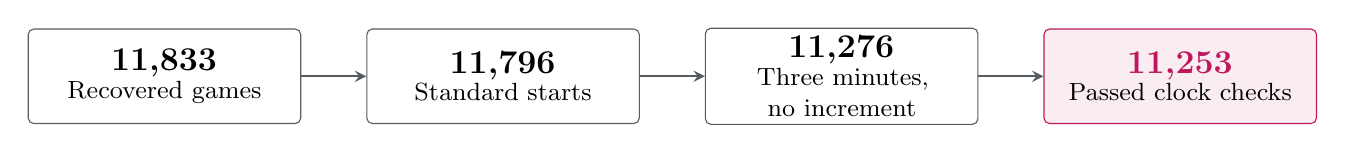
\begin{tikzpicture}[
  stage/.style={draw=CityUMuted,rounded corners=2pt,minimum height=1.2cm,
               text width=3.25cm,align=center,inner sep=3pt,font=\small},
  flow arrow/.style={->,>=stealth,thick,CityUMuted}]
\node[stage] (original) at (0,0) {\large\bfseries\RecoveredGames\\[-1pt]\normalfont\small Recovered games};
\node[stage] (standard) at (4.3,0) {\large\bfseries\StandardStartGames\\[-1pt]\normalfont\small Standard starts};
\node[stage] (control) at (8.6,0) {\large\bfseries\TimeControlGames\\[-1pt]\normalfont\small Three minutes, no increment};
\node[stage,draw=CityUAccent,fill=CityUTint] (verified) at (12.9,0) {\large\bfseries\textcolor{CityUAccent}{\VerifiedGames}\\[-1pt]\normalfont\small Passed clock checks};
\draw[flow arrow] (original) -- (standard);
\draw[flow arrow] (standard) -- (control);
\draw[flow arrow] (control) -- (verified);
\end{tikzpicture}
\caption{Sequential selection of September 2026 games. The \VerifiedGames{} retained games contained \RebuiltMoves{} individual moves, of which \VerifiedMoves{} had finite engine scores before and after the move. Table~\ref{tab:sample} gives the exclusions.}\label{fig:cohort}
\end{figure}

The archived move table contained 953,174 rows. Removing 25,872 exact duplicates and retaining labelled moves yielded 913,510 observations from 11,812 games. Consecutive engine evaluations reproduced the archived label for all 903,656 moves with both records available. We checked the timing of the clock readings separately.

\clearpage
\section{Clock reconstruction and evaluation design}
We aligned the archived clock fields with the public move records. For \emph{all} 913,510 labelled moves, the field labelled as the opponent's clock equalled the mover's clock \emph{after} the move. This value coincided with the opponent's actual pre-move time on only 15,478 moves. The extraction code read the next clock entry in the sequence (Figure~\ref{fig:audit}). It also pooled successive turns by both players when computing recent time use.

We initialised each clock at 180 seconds and reconstructed its pre-move value from that player's last completed turn. At the corrected index, all 926,332 comparable readings agreed with the rounded timestamps in the annotated game records to within half a second. At the archived index, 52,856 readings (5.71\%) met this tolerance. Before fitting any models, we excluded games in which either clock increased by more than one second between successive readings for the same player, including the first reading relative to 180 seconds. The verified sample contained 69,799 serious errors in \VerifiedMoves{} labelled moves (\VerifiedPrevalence\%).

\begin{figure}[H]\centering
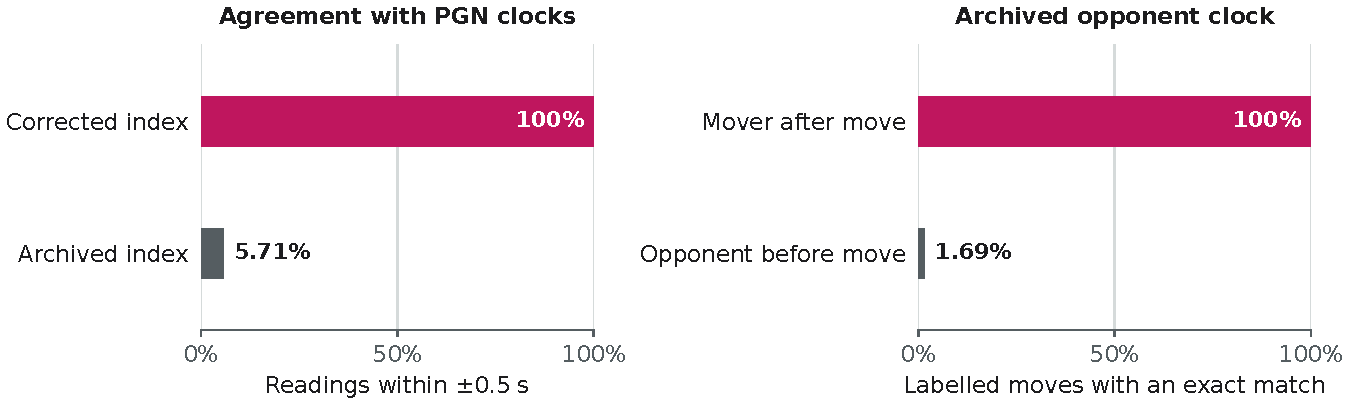
\includegraphics[width=.94\linewidth,height=6.6cm,keepaspectratio]{../../results/model_comparison/report_figures/clock_alignment.pdf}
\caption{Clock alignment against the original game records. The comparison to Portable Game Notation (PGN) timestamps allows for rounding to the nearest second (926,332 readings). The archived-field comparison tests exact agreement on 913,510 labelled moves. A move can satisfy both exact-match checks if the readings coincide.}\label{fig:audit}
\end{figure}

\subsection{Nested feature sets and temporal validation}
The baseline feature set includes both players' ratings, move number, side to move, material, game phase, number of legal moves, check status and the pre-move engine evaluation. The second set adds both pre-move clocks and the mover's share of their combined time. The third adds the duration of the mover's preceding turn and the mean duration of their last one to three completed turns. We refitted histogram gradient boosting for each feature set. Equation~\eqref{eq:outcome} implies that a ten-point drop is impossible when \(W(c_{\rm before})<10\). We therefore set the predicted probability to zero for those moves. This zero-risk rule applied to 45,606 labelled moves, including \EligibleTest{} in the final week. None met the error threshold.

Missing own-turn durations were set to zero with a history-missing indicator. Both clocks were transformed by \(\log(1+t)\). All fitted models received the same cubic spline bases with four knots, standardised linear terms and phase indicators for their input set. The clock input sets also included clock-by-rating and clock-by-phase interactions. Knot placement, scaling and constant-column removal used each training window only; standardised linear values were clipped to \([-10,10]\).

\begin{table}[H]\centering
\caption{Chronological training and evaluation windows in September 2026 (UTC). Each split assigns complete games to the training or evaluation period.}\label{tab:windows}
\begin{tabular}{@{}ccc@{}}\toprule
Stage & Training days & Evaluation days \\\midrule
Development window 1 & 1--8 & 9--13 \\
Development window 2 & 1--13 & 14--18 \\
Development window 3 & 1--18 & 19--23 \\
Refit and final-week evaluation & 1--23 & 24--30 \\\bottomrule
\end{tabular}
\end{table}

In each window of Table~\ref{tab:windows}, we fitted the preprocessing steps on the training days and evaluated predictions on later games. We selected the model with the lowest mean validation log loss, giving each of the three windows equal weight. Log loss penalises confident errors more heavily. We refitted the selected model on 642,668 moves from 8,621 games and evaluated it on \VerifiedTestMoves{} moves from \VerifiedTestGames{} other games. As the earlier study had already evaluated the final week, this comparison reuses that evaluation period. To estimate uncertainty in loss differences, we paired predictions on each move and drew 1,000 bootstrap samples of whole games with replacement. For validation, we resampled within each window before averaging across windows.

\clearpage
\subsection{Incremental value of pre-move clocks and recent time use}
\begin{figure}[H]\centering
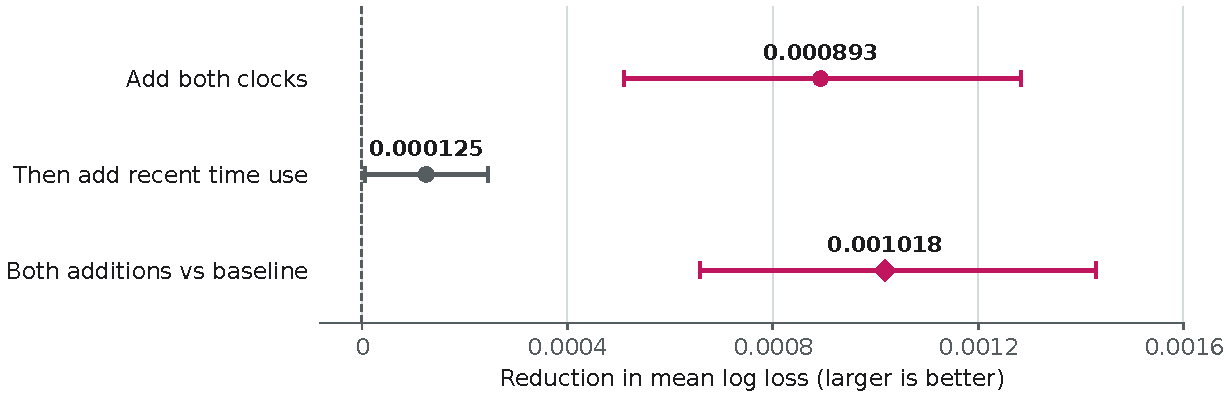
\includegraphics[width=.94\linewidth,height=6.6cm,keepaspectratio]{../../results/model_comparison/report_figures/feature_gains.pdf}
\caption{Reduction in mean log loss on 196,508 final-week moves. Positive values indicate improvement. The third estimate compares the full model directly with the position-and-ratings baseline. Intervals are the 2.5th and 97.5th percentiles of 1,000 paired bootstrap resamples of 2,632 games. Table~\ref{tab:increments} gives the absolute losses.}\label{fig:gains}
\end{figure}
Adding both pre-move clocks reduced final-week log loss by 0.000893 from the position-and-ratings baseline of \BoardOnlyTest{} (Figure~\ref{fig:gains}). Adding recent time use yielded a further reduction of 0.000125 (Table~\ref{tab:increments}). The combined reduction was 0.001018 (95\% paired bootstrap interval, 0.000658 to 0.001429). With the predictors added in this order, the two clocks accounted for about 88\% of the reduction. The corresponding mean reductions across the development windows were 0.001075 and 0.000199, respectively.


\section{Model selection and predictive performance}
We compared L2-regularised logistic regression, histogram gradient boosting and a fixed XGBoost configuration against a constant predictor based on the training error rate. The logistic model uses spline terms for clock time, rating and move number, with interactions between clock time and both rating and game phase. The tree models estimate interactions through successive splits. The original development search evaluated four logistic penalty settings and five histogram gradient boosting configurations. We retained \(C=1\) for logistic regression. For histogram gradient boosting, we used 250 iterations, a learning rate of 0.05, up to 31 leaves, at least 100 observations per leaf and an L2 penalty of 10~\cite{sklearn}. XGBoost used 250 trees with a maximum depth of five, a learning rate of 0.05, a minimum child weight of five and an L2 penalty of 10~\cite{xgboost}.

\begin{figure}[H]\centering
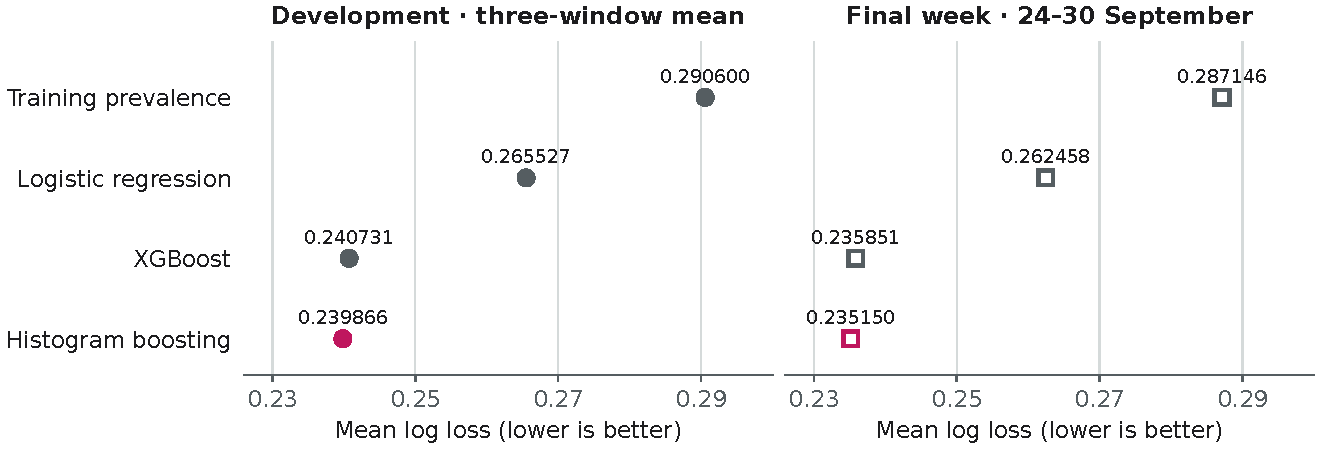
\includegraphics[width=.94\linewidth,height=5.85cm,keepaspectratio]{../../results/model_comparison/report_figures/model_comparison.pdf}
\caption{Mean log loss for each model on the three development windows and the previously evaluated final week. The constant model predicts the training prevalence. The other models use the full feature set and the zero-risk rule. Table~\ref{tab:revised} includes the corresponding unconstrained fits and secondary metrics.}\label{fig:models}
\end{figure}

Histogram gradient boosting with the zero-risk rule achieved the lowest mean validation log loss (\SelectedValidation{}, Figure~\ref{fig:models}). The rule reduced final-week log loss by 0.004932 for logistic regression and by 0.000012 for histogram gradient boosting. The smaller reduction reflects the low probabilities the trees already assigned to these positions. With the rule applied to both tree models, final-week log loss for the fixed XGBoost configuration exceeded that for histogram gradient boosting by 0.000702 (95\% paired bootstrap interval, 0.000462 to 0.000938).

\clearpage
\subsection{Calibration by predicted-risk decile}
The final week contained 16,401 serious errors in \VerifiedTestMoves{} moves (\VerifiedTestRate\%). To assess calibration, we grouped moves into deciles of predicted risk (Figure~\ref{fig:calibration}). In the highest-risk decile (19,651 moves), the mean predicted probability was 28.12\% and the observed error rate was 28.87\%, more than three times the overall rate. The absolute difference between the mean prediction and the observed rate was less than one percentage point in every decile. The largest difference was 0.91 percentage points. These group averages describe calibration in this evaluation sample.

\begin{figure}[H]\centering
\begin{tikzpicture}
\begin{axis}[width=9.5cm,height=6.7cm,xmin=0,xmax=31,ymin=0,ymax=31,
 xtick={0,5,10,15,20,25,30},ytick={0,5,10,15,20,25,30},
 xlabel={Mean predicted error probability (\%)},ylabel={Observed serious errors (\%)},
 tick label style={font=\small},label style={font=\small},tick align=outside,
 axis lines=left,axis line style={black!65},legend cell align=left,
 legend style={font=\small,draw=none,at={(.03,.98)},anchor=north west}]
\addplot[gray,dashed,domain=0:31,samples=2]{x};
\addlegendentry{Perfect calibration}
\addplot[only marks,mark=*,mark size=2.1pt,color=CityUAccent]
 table[col sep=comma,x expr={100*\thisrow{predicted_probability}},y expr={100*\thisrow{observed_rate}}]
 {../../results/model_comparison/verified_180_0/selected_calibration.csv};
\addlegendentry{Histogram boosting with zero-risk rule}
\end{axis}\end{tikzpicture}
\caption{Calibration of the selected model on 24--30 September. Each point represents a predicted-risk decile (approximately 19,650 moves). Points above the diagonal indicate underestimation of the observed error rate.}\label{fig:calibration}
\end{figure}
The selected model achieved a Brier score (mean squared probability error) of 0.06815 and an area under the ROC curve (ROC AUC) of \BestAUC{}. Average precision (AP) was \BestAP{}, compared with a final-week error prevalence of 0.0835.

\section{Clock information across game phases and rating bands}
\subsection{Observed error rates by phase}
We classified moves 1--10 as the opening. For subsequent moves, we classified positions with at most 14 points of non-pawn material as endgames and all remaining positions as middlegames. Across the month, serious errors occurred on 2.96\% of opening moves, 10.98\% of middlegame moves and 6.55\% of endgame moves. Figure~\ref{fig:phaserates} gives the corresponding rates on the final week. Middlegames had the highest observed error rate. This sets the context for the next comparison, which asks how much the clocks improve the forecast within each phase.

\begin{figure}[H]\centering
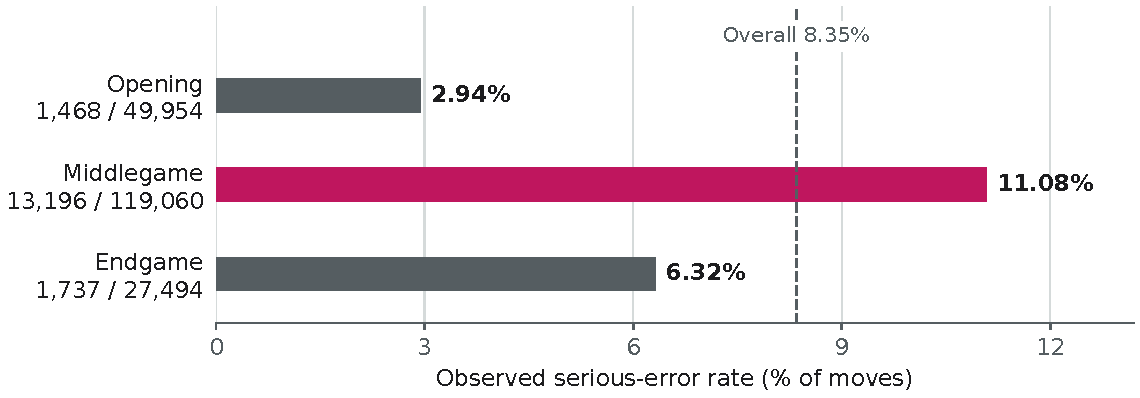
\includegraphics[width=.94\linewidth,height=6.15cm,keepaspectratio]{../../results/model_comparison/report_figures/phase_error_rates.pdf}
\caption{Observed serious-error rates by game phase on 24--30 September. Denominators are individual moves. The overall rate is the move-weighted proportion across the three phases.}\label{fig:phaserates}
\end{figure}

\clearpage
\subsection{Log-loss reductions within subgroups}
During the final week, the two pre-move clocks reduced log loss by 0.000585 in the opening, 0.000733 in the middlegame and 0.002147 in the endgame (Figure~\ref{fig:subgroup}). Endgames had the largest estimated reduction, based on 27,494 moves. For players rated below 1600, the estimated reduction also favoured the clocks, although the interval included zero. These within-group intervals do not test differences between groups.
% Whole-game bootstrap estimates, prepared by scripts/clock_subgroups.py.
% Rows are the full sample, the three game phases, then the three rating bands.
\begin{figure}[H]
\centering
\begin{tikzpicture}
\begin{axis}[
 width=.83\linewidth,height=7cm,
 axis x line*=bottom,axis y line*=left,y axis line style={draw=none},ytick style={draw=none},tick align=outside,
 ymin=.35,ymax=7.7,ytick={1,2,3,4,5,6,7},
 yticklabels={Rating at least 2200,Rating 1600--2199,Rating below 1600,
 Endgame,Middlegame,Opening,All moves},
 yticklabel style={font=\small},yticklabel pos=left,ytick pos=left,
 xticklabel style={font=\footnotesize},xlabel style={font=\small},
 xlabel={Reduction in mean log loss \((\times 10^{-3})\)},
 enlarge x limits=.10,
 legend style={font=\footnotesize,draw=none,at={(.5,1.02)},anchor=south,
  /tikz/every even column/.append style={column sep=8pt}},
 legend columns=2,legend cell align=left]
\addplot[only marks,mark=*,mark size=1.9pt,line width=.75pt,
 color=CityUAccent,
 error bars/.cd,x dir=both,x explicit,error bar style={line width=.6pt}]
 table[col sep=comma,x expr={-1000*\thisrow{clock_delta}},
 y expr={7-\coordindex+.13},
 x error minus expr={1000*(\thisrow{clock_upper}-\thisrow{clock_delta})},
 x error plus expr={1000*(\thisrow{clock_delta}-\thisrow{clock_lower})}]
 {\subgrouppath};
\addlegendentry{Add pre-move clocks}
\addplot[only marks,mark=triangle*,mark size=2.3pt,line width=.75pt,
 color=CityUMuted,
 error bars/.cd,x dir=both,x explicit,error bar style={line width=.6pt}]
 table[col sep=comma,x expr={-1000*\thisrow{history_delta}},
 y expr={7-\coordindex-.13},
 x error minus expr={1000*(\thisrow{history_upper}-\thisrow{history_delta})},
 x error plus expr={1000*(\thisrow{history_delta}-\thisrow{history_lower})}]
 {\subgrouppath};
\addlegendentry{Then add recent time use}
\draw[gray,densely dashed] (axis cs:0,.5) -- (axis cs:0,7.55);
\end{axis}
\end{tikzpicture}
\caption{Reduction in mean log loss after adding pre-move clocks and then recent time use, 24--30 September. Points to the right of zero indicate improvement. The 95\% intervals use 1,000 paired bootstrap resamples of whole games within each subgroup. Games may contribute to several subgroups. The intervals are exploratory and unadjusted for multiple comparisons.}\label{fig:subgroup}
\end{figure}


\subsection{Adjusted error probability by remaining time}
We used logistic regression with the zero-risk rule to estimate how predicted error probability varied with remaining time. Within each phase and rating band, we set the mover's clock in turn to its 10th, 25th, 50th, 75th and 90th percentiles, recalculating the clock share and interaction terms at each value. We held the other predictors at their observed values and averaged the resulting probabilities over positions in that subgroup (Figure~\ref{fig:adjusted}).
\begin{figure}[H]\centering
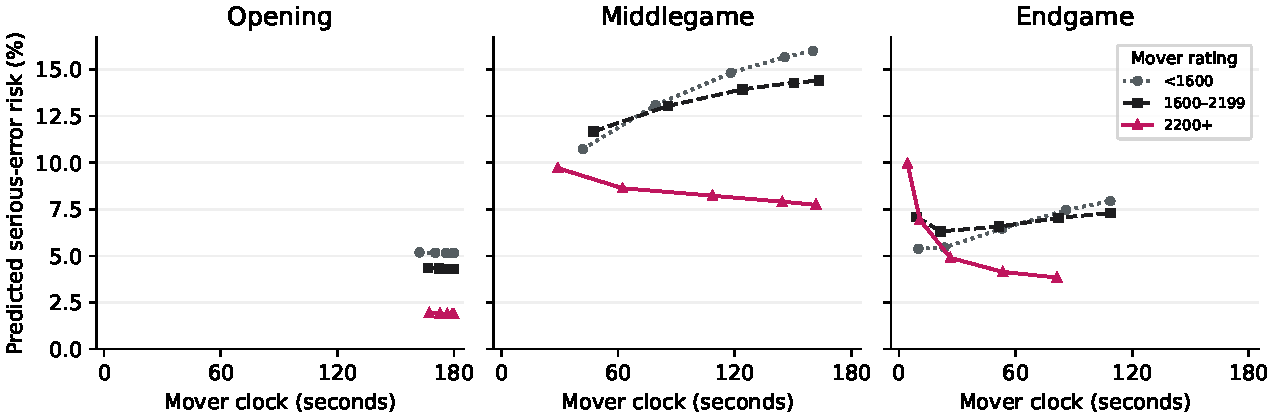
\includegraphics[width=.94\linewidth,height=6.5cm,keepaspectratio]{../../results/model_comparison/adjusted_clock_curves.pdf}
\caption{Adjusted probabilities of serious error from logistic regression, 24--30 September. Each curve uses the observed clock percentiles and distribution of positions in its phase and rating band.}\label{fig:adjusted}
\end{figure}
In endgames involving movers rated at least 2200, the adjusted probability of a serious error fell from 9.93\% at 4.4 seconds to 3.84\% at 81.4 seconds. For movers rated below 1600, it rose from 5.38\% at 10.0 seconds to 7.94\% at 108.8 seconds. Opening clock readings clustered near 180 seconds. The clocks improved overall prediction even though the fitted relationship between remaining time and error probability varied by phase and rating. These profiles are descriptive averages from the fitted logistic model. Setting a clock while holding the other inputs fixed can create clock-history combinations absent from the observed games.

\clearpage
\section{Sensitivity analyses and generalisability}
The development and final-week samples shared 639 players. We held the evaluation sample fixed and removed every training game involving a final-week player. This left 509 training games and 33,737 moves (5.25\% of the original training moves). Final-week log loss rose from 0.23515 to 0.24605 (Table~\ref{tab:robust}). Because the restriction reduced the training sample and changed its player composition, the increase cannot be attributed solely to the absence of familiar players.

\begin{table}[H]\centering
\caption{Sensitivity to player overlap and outcome definition in verified \(180+0\) games, 24--30 September. The final two rows use the pre-move winning-chance score \(W\) as a predictor.}\label{tab:robust}
\begin{tabular}{@{}cccccc@{}}\toprule
Outcome or training restriction & Train moves & Test moves & Event rate (\%) & Log loss & AP \\\midrule
\RobustRows
\bottomrule\end{tabular}
\end{table}
A five-percentage-point threshold classified 16.28\% of final-week moves as serious errors, compared with 5.10\% at a fifteen-point threshold. Assigning forced mates to the endpoints of the winning-chance scale expanded the evaluation sample to 205,411 moves and changed the error prevalence.

\subsection*{Interpretation and limitations}
On the same 196,508 final-week moves, adding pre-move clocks and recent time use reduced log loss by 0.001018 (95\% paired whole-game bootstrap interval, 0.000658 to 0.001429), a relative reduction of 0.43\%. With inputs added in this order, the starting clocks accounted for 87.70\% of the gain. Recent time use supplied a smaller additional improvement. The full model's predicted and observed event rates differed by less than one percentage point in every risk decile, describing group-level calibration in this sample.

The player-disjoint model retained only 5.25\% of the training moves and had a higher log loss. Training size and player composition changed together, so the comparison combines their effects. A difficult position may require more time and also increase the risk of error. The observed predictive gain alone cannot establish how allocating more time would change a player's error risk.

The sampling design favours active players whose games have public engine annotations. Without an unfiltered comparison sample, we cannot estimate site-wide error prevalence. The game-level bootstrap preserves dependence among moves in the same game, but repeated players may also induce dependence across games. The final week had already been examined in the earlier analysis. Evaluation on a new month would provide an independent test of calibration and of the incremental value of pre-move clocks.

Appendix~\ref{app:reproducibility} documents the code, data and archived benchmark. Appendix~\ref{app:numerical} gives exact counts and model scores for the figures.

\begin{thebibliography}{9}\small\raggedright\setlength{\itemsep}{1pt}\setlength{\parskip}{0pt}
\bibitem{maia} R. McIlroy-Young, S. Sen, J. Kleinberg and A. Anderson. Aligning superhuman AI with human behavior: Chess as a model system. \emph{KDD}, 2020. \href{https://arxiv.org/abs/2006.01855}{arXiv:2006.01855}.
\bibitem{lichessapi} Lichess. Game export API. \href{https://lichess.org/api#tag/Games}{API documentation}.
\bibitem{lichesswin} Lichess. Accuracy metric. \url{https://lichess.org/page/accuracy}.
\bibitem{sklearn} F. Pedregosa et al. Scikit-learn: Machine learning in Python. \emph{Journal of Machine Learning Research}, 12, 2825--2830, 2011. \href{https://www.jmlr.org/papers/v12/pedregosa11a.html}{Publisher's record}.
\bibitem{xgboost} T. Chen and C. Guestrin. XGBoost: A scalable tree boosting system. \emph{KDD}, 2016. \href{https://doi.org/10.1145/2939672.2939785}{doi:10.1145/2939672.2939785}.
\end{thebibliography}
\clearpage
\appendix
\counterwithin{table}{section}
\refstepcounter{section}\label{app:reproducibility}
\section*{Appendix \thesection. Project materials and reproducibility}
\addcontentsline{toc}{section}{Appendix \thesection. Project materials and reproducibility}

\subsection{Repository and data provenance}
The group repository is \url{https://github.com/CanyonChen/Beyond-the-Board}. The
\href{https://github.com/CanyonChen/Beyond-the-Board/tree/92dd2e7c60d5f3efc5950686f538bdd42e310a98}{archived revision \texttt{92dd2e7}}
contains the original mixed-blitz move table and benchmark scores. The source-verified analysis, revised figures and fitted model accompany this report in the local project. All paths below are relative to its root.

Game IDs in \path{data/moves.csv.gz} identify the original sample. We recovered the corresponding public move records through the \href{https://lichess.org/api#tag/Games}{Lichess game export API}. The reconstructed table, \path{data/processed/moves_verified.csv.gz}, retains all 888,993 moves from the eligible games. Of these, 839,176 have the two finite engine evaluations needed for the primary outcome. Each player starts with 180 seconds. The previous-turn duration and rolling mean are initially missing for that player and become available as their own turns accumulate.

\path{data/processed/recovery_counts.json} records sequential exclusions and both the compressed and uncompressed data checksums. The SHA-256 digest below identifies the compressed table used in the model comparison.
\begin{center}\small\ttfamily
9faf8fd13a2196d4daad9491baa4c1fb735e0cc46a0de7793c206a87a41a554b
\end{center}
The timestamp alignment checks are in \path{data/processed/clock_audit.json}. The source-recovery commands and definitions of each move-level field are in \path{data/README_data.md}.

\subsection{Reproducing and interpreting the estimates}
Starting from the supplied move tables, run the following commands from the project root in a Python environment. The verified run used Python~3.13.15, scikit-learn~1.9.1 and XGBoost~3.4.1.
{\small
\begin{verbatim}
python -m pip install -r requirements.txt
python scripts/reproduce_baselines.py
python scripts/compare_models.py --input data/processed/moves_verified.csv.gz --history provided
python scripts/clock_subgroups.py tmp/clock_predictions.csv.gz results/model_comparison/clock_subgroups.csv
\end{verbatim}
}
The modelling outputs are in \path{results/model_comparison/verified_180_0/}.
\path{selection.json} identifies the input digest, model settings and software versions. The three development windows and the reused final week can be checked in \path{fold_metrics.csv}. For each contrast, \path{paired_log_loss.csv} records the signed difference and the 2.5th and 97.5th percentiles of 1,000 paired, whole-game bootstrap resamples. For example, \texttt{clocks\_minus\_no\_time} subtracts the loss of the position-and-ratings model from the loss after adding both clocks. Its final-week value is \(-0.000893\), equivalent to a reduction of \(0.000893\). \path{selected_calibration.csv} supplies the counts and observed and predicted probabilities for the calibration plot.

With the supplied result tables in place, run \texttt{python scripts/plot\_report\_figures.py} to regenerate the clock-alignment, feature-gain, model-comparison and phase-specific error-rate plots. The source mapping and export details accompany the vector figures in \path{results/model_comparison/report_figures/manifest.json}. The project \path{README.md} gives the commands for the adjusted clock curves, sensitivity analyses, saved-model inference and report build.

\subsection{Reproduction of the archived benchmark}
Refitting the archived models reproduced the ranking in Table~\ref{tab:baseline}. Final-week log loss for histogram gradient boosting was 0.231266 in the replication and 0.231271 in the archive. Removing the archived clock readings and recent time use increased log loss by 0.00446. The archived clock fields included post-move information, so this difference cannot quantify the predictive value of the pre-move clocks.
\begin{table}[H]\centering
\caption{Archived mixed-blitz benchmark on 24--30 September (213,295 moves, 2,752 games). Differences in clock alignment and sample composition limit direct comparison with Table~\ref{tab:revised}.}\label{tab:baseline}
\begin{tabular}{@{}ccccc@{}}\toprule
Model & Log loss & Brier score & ROC AUC & AP \\\midrule
Training prevalence & 0.28781 & 0.07673 & 0.5000 & 0.0837 \\
L2 logistic regression & 0.26660 & 0.07369 & 0.7082 & 0.1672 \\
Histogram gradient boosting & 0.23127 & 0.06737 & 0.8235 & 0.2800 \\\bottomrule
\end{tabular}
\end{table}

\clearpage
\refstepcounter{section}\label{app:numerical}
\section*{Appendix \thesection. Numerical results behind the figures}
\addcontentsline{toc}{section}{Appendix \thesection. Numerical results behind the figures}

\subsection{Sample selection}
Figure~\ref{fig:cohort} counts games through three sequential eligibility checks. The last row below switches to the move-level labelling criterion. A finite score is required on both sides of an observed move.

\begin{table}[H]\centering
\caption{Selection of the September 2026 analysis sample. Counts reflect sequential exclusions.}\label{tab:sample}
\begin{tabular}{@{}ccc@{}}\toprule
Selection step & Games remaining & Moves or labels \\\midrule
Recovered from the original collection & 11,833 & --- \\
Exclude 37 games with nonstandard starting positions & 11,796 & --- \\
Exclude 520 remaining games with other time controls & 11,276 & --- \\
Exclude 23 games with unexplained clock increases & \VerifiedGames & 888,993 moves \\
Require finite engine scores before and after the move & \VerifiedGames & \VerifiedMoves{} labels \\\bottomrule
\end{tabular}
\end{table}

\subsection{Incremental value of time information}
Each row adds predictors to the row above. Figure~\ref{fig:gains} shows reductions in log loss as positive values. The final column below reports the signed change (augmented model minus preceding model), so a negative change means an improvement.

\begin{table}[H]\centering
\caption{Incremental value of clock information in verified \(180+0\) games. The final column gives the change in log loss from the preceding row for 24--30 September, with a 95\% paired game-level bootstrap interval. Negative values indicate lower loss.}\label{tab:increments}
\begin{tabular}{@{}cccc@{}}\toprule
Inputs & Validation log loss & Final-week log loss & Change [95\% interval] \\\midrule
\IncrementRows
\bottomrule\end{tabular}
\end{table}

\subsection{Model comparison and probability metrics}
Figure~\ref{fig:models} compares the constant baseline and the three model families with the zero-risk rule applied to the trained models. The table also gives their unconstrained counterparts. Lower log loss and Brier scores indicate better probability forecasts. Higher ROC AUC and average precision (AP) indicate better discrimination.
 
\begin{table}[H]\centering
\caption{Predictive performance on verified \(180+0\) games. Validation log loss is the mean across three development windows. The remaining metrics cover 24--30 September. Bold indicates the model selected by validation log loss.}\label{tab:revised}
\begin{tabular}{@{}cccccc@{}}\toprule
Model & \shortstack{Validation\\log loss} & \shortstack{Final-week\\log loss} & Brier score & ROC AUC & AP \\\midrule
\PerformanceRows
\bottomrule\end{tabular}
\end{table}

\end{document}
